The system consists of three logically separate components as illustrated in
Figure~\ref{fig:system_overview}; 1) the equipment component where all
communication with equipment and acquisition of data is performed 2) the
servers which consist of the MySQL server that stores the acquired data from
experiments and the Apache webserver which interacts and presents the user with
data retrieved from the database and 3) the user component which consists of
the clients wishing to access the data. 

\begin{figure}
 \begin{center}
 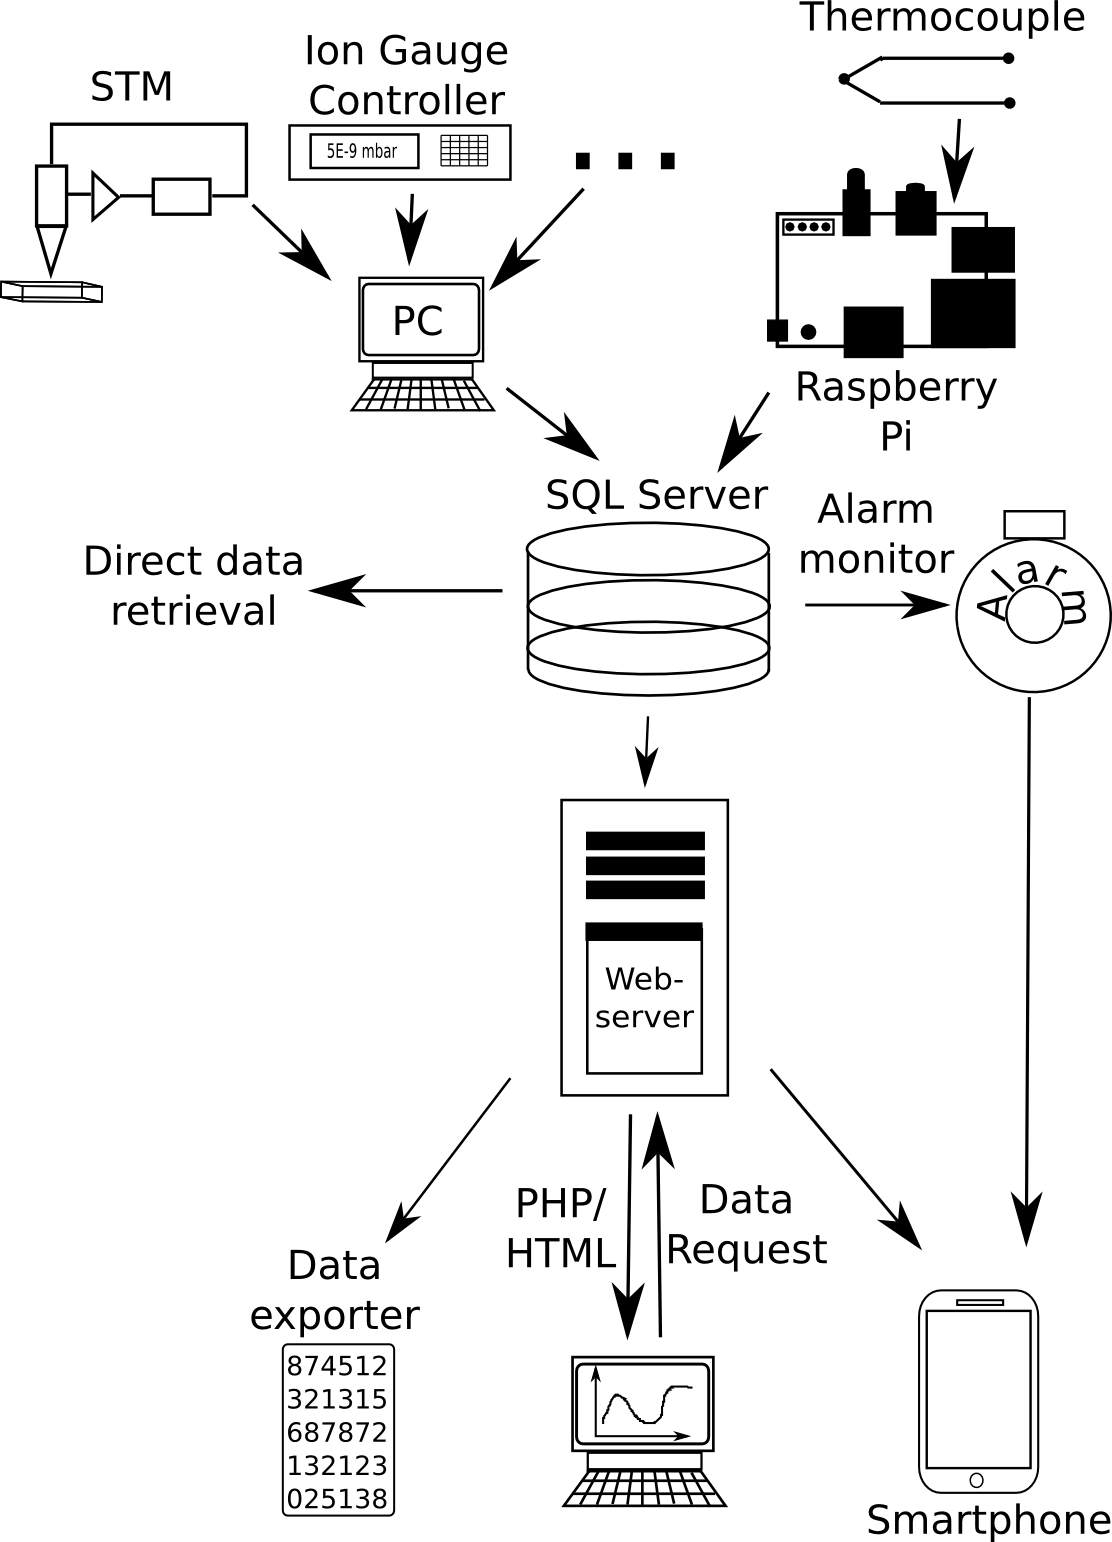
\includegraphics[width=10cm]{system_overview.png}
 \caption{
   A schematic representation of the structure of data handling system.
   \label{fig:system_overview}
 } 
 \end{center}
\end{figure}

The system is highly flexible meaning the servers can accept data from a range
of different sources. In the current setup equipment interfaced with RS232,
GPIB, USB and analog/digital data acquisition cards standards are logged to the
MySQL database. The user can furthermore use programs written in a wide variety
of languages. As a testimony to this, software written in both LabView and
Python\cite{python} are used to save data to the database. How the integration
with the server and subsequent storage of data in the database is performed is
hence a user determined design decision. This has a number of advantages.  The
user(s) can integrate existing software with the databases quickly and without
the need to rewrite any previous interface software written for experimental
setups. Furthermore, due to the flexibility of the system, if storage in the
database during acquisition is not possible due to software limitations the
data can still be saved in the database by subsequent post experiment parsing
of data files. This, however, still requires that the file format, which holds
the data, is specified or the data can be exported to a flat text format from
the acquisition software.

The servers consist of a MySQL server and a web server. All experimental data
acquired by the user is stored in the MySQL database and is presented to the
user from the web server. If needed, experimental data from the MySQL server
can be retrieved directly for later analysis. The web server runs a LAMP
(Linux, Apache, MySQL, PHP/Python) package. Python, PHP and HTML/CSS and is
used to extract data from the database and present them to the end user in a
simple interactive web interface for data visualization and simple treatment
algorithms. Python was primarily chosen due to its tight integration with
scientific packages, such as SciPy and NumPy, which makes data analysis and
treatment more convenient\cite{Cahn2007}. PHP and HTML/CSS is used to display
data in standardized formats suitable for web browsers and process input from
the user. The combination of PHP and HTML/CSS to process user input from web
pages is very flexible and has proven successful in other parts of the
scientific community\cite{Crane2008}. To accommodate a range of users and
provide the largest flexibility the web server displays both a standard HTML/CSS
site for desktop PCs and a mobile version suitable for tablet/smartphone users.


The web interface, which takes user input and displays data to the user, is also
capable of routine data treatment. This can either be zoom of data, plotting on
a log scale, performing a running average, etc. The data treatment is easily
extendable allowing the user to add any function necessary. In this way the
user can easily and quickly get an overview of acquired data.
